\documentclass[a4paper,12pt,oneside]{book}

%-------------------------------Start of the Preamble------------------------------------------------
\usepackage[english]{babel}
\usepackage{blindtext}
\usepackage{graphicx}
\usepackage{tikz}
\usepackage{hyperref}
\usetikzlibrary{positioning}
\usetikzlibrary{shapes.geometric, arrows}
%package for hyperlinks
\usepackage{hyperref}
\hypersetup{
    colorlinks=true,
    linkcolor=blue,
    filecolor=magenta,      
    urlcolor=cyan,
}

\urlstyle{same}
%use of package fancy header
\usepackage{fancyhdr}
\setlength\headheight{26pt}
\fancyhf{}
%\rhead{\includegraphics[width=1cm]{logo}}
\lhead{\rightmark}
\rhead{\includegraphics[width=1cm]{logo}}
\fancyfoot[RE, RO]{\thepage}
\fancyfoot[CE, CO]{\href{http://www.e-yantra.org}{www.e-yantra.org}}

\pagestyle{fancy}
\renewcommand{\thesection}{\arabic{section}}





%use of package for section title formatting
\usepackage{titlesec}
\titleformat{\chapter}[display]
  {\Large\bfseries\raggedright} % format
  {}                % label
  {0pt}             % sep
  {\huge}           % before-code

% Adjust spacing before section headings
\titleformat{\section}[block]
  {\normalfont\Large\bfseries\raggedright}{\thesection}{1em}{}
\titlespacing*{\section}{0pt}{\baselineskip}{\baselineskip}

\titleformat{\subsection}[block]
  {\normalfont\large\bfseries\raggedright}{\thesubsection}{1em}{}
\titlespacing*{\subsection}{0pt}{\baselineskip}{\baselineskip}

\titleformat{\subsubsection}[block]
  {\normalfont\normalsize\bfseries\raggedright}{\thesubsubsection}{1em}{}
\titlespacing*{\subsubsection}{0pt}{\baselineskip}{\baselineskip}

%use of package tcolorbox for colorful textbox
\usepackage[most]{tcolorbox}
\tcbset{colback=cyan!5!white,colframe=cyan!75!black,halign title = flush center}

\newtcolorbox{mybox}[1]{colback=cyan!5!white,
colframe=cyan!75!black,fonttitle=\bfseries,
title=\textbf{\Large{#1}}}

%use of package margin note for notes in the margin
\usepackage{marginnote}

%use of package watermark for pages
%\usepackage{draftwatermark}
%\SetWatermarkText{\includegraphics{logo}}
\usepackage[scale=2,opacity=0.1,angle=0]{background}
\backgroundsetup{
contents={\includegraphics{logo}}
}

%use of new command for keywords color
\usepackage{xcolor}
\newcommand{\keyword}[1]{\textcolor{red}{\textbf{#1}}}

%package for inserting pictures
\usepackage{graphicx}

%package for highlighting
\usepackage{soul}

%new command for the table
\newcommand{\head}[1]{\textnormal{\textbf{#1}}}

%package for adjusting hyphenation
\usepackage{hyphenat}
\usepackage{ragged2e}
\usepackage{etoolbox}

\apptocmd{\sloppy}{\hbadness 10000\relax}{}{}

%----------------------End of the Preamble---------------------------------------

\begin{document}

%---------------------Title Page------------------------------------------------
\begin{titlepage}
\raggedright
{\Large e-YSIP 2023\\[1cm]}
{\Huge\scshape The Collective AI \\[.1in]}
\vfill
\begin{flushright}
{\large Riya Gupta \\}
{\large Valhari Meshram \\}
{\large Sri Venkateshwar \\}
{\large Mentor: Shyama \\}
{\large Duration of Internship: $ 22/05/2023 - 07/07/2023 $ \\}
\end{flushright}

{\itshape 2023, e-Yantra Publication}
\end{titlepage}
%-------------------------------------------------------------------------------

\section[Abstract]{The Collective AI}
\section*{Abstract}
This technical documentation provides a detailed overview of the summer internship project titled "The Collective AI". The project aims to develop two autonomous robots capable of navigating a black-and-white line grid in an arena. The robots employ IR sensors for line following and object recognition to identify specific objects placed within the arena. Upon detection, the robots compare the objects with a custom label database and proceed to pick them up and place them at desired positions. The project addresses challenges in object recognition accuracy, communication and coordination between the robots, and efficient pick-and-place functionality.

\tableofcontents
\newpage
\section{Introduction}
The Collective AI project aims to develop a system consisting of two autonomous robots capable of navigating a black-and-white line grid in an arena. These robots utilize IR sensors for line following and object recognition to accurately identify specific objects placed within the arena. The project addresses challenges related to object recognition accuracy, communication and coordination between the robots, and the development of efficient pick-and-place functionality. By combining expertise in software and hardware components, the project aims to create a comprehensive solution for robot construction, line following mechanisms, object recognition processes, communication and coordination setups, pick-and-place mechanisms, and future work. Notable achievements include the successful development of a custom object detection model for accurate object identification and classification, the implementation of line following using an array of IR sensors, the design, and development of custom robots, the establishment of communication among various robot components and inter-robot communication, as well as the creation of sophisticated pick-and-place mechanisms. Synchronization and coordination between the robots have been prioritized to avoid collisions within the arena. With the goal of achieving autonomous navigation, accurate object identification, and reliable pick-and-place operations, the Collective AI project aims to overcome challenges related to object recognition, communication, and pick-and-place functionality.Applications include autonomous navigation, accurate object identification, and reliable pick-and-place operations, addressing challenges in object recognition, communication, and pick-and-place functionality.
The concept has industrial applications in automation, robotics, and smart manufacturing. It can be used for warehouse automation, manufacturing assembly lines, quality control, logistics, agriculture, hazardous environment inspections, smart retail, and healthcare. The project integrates custom object detection, IR sensor-based line following, and pick-and-place mechanisms for efficient and reliable operations.
\newpage
\section{Software and Hardware Components}
The Collective AI project utilizes a combination of software and hardware components to achieve its objectives.

\subsection{Software}
\begin{itemize}
  \item Embedded C++: Programming language used for firmware development.
  \item Python: Utilized for image processing and object recognition.
  \item Arduino IDE: Integrated Development Environment for programming the Arduino Uno and ESP32 Camera module.
  \item OpenCV: Machine learning framework for training object recognition models.
\end{itemize}

\section*{Component Specifications}


\subsection*{ESP 32 Camera Module $^[^1^]$}
\href{https://media.digikey.com/pdf/Data%20Sheets/DFRobot%20PDFs/DFR0602_Web.pdf}{Datasheet}
\begin{itemize}
  \item Microcontroller: ESP32
  \item Image Sensor: OV2640
  \item Maximum Resolution: 2 Megapixels
  \item Operating Voltage: 3.3V
  \item Communication: Wi-Fi and Bluetooth
  \item GPIO Pins: Available for general-purpose use
  \item Supported Formats: JPEG, BMP, RGB565, YUV, and more
  \item Additional Features: Camera interface, SD card slot, and onboard flash memory
\end{itemize}

\subsection*{L298N Dual H-Bridge Motor Controller $^[^2^]$}
\href{https://www.etechnophiles.com/l298n-motor-driver-pin-diagram/}{Datasheet}
\begin{itemize}
  \item Motor Driver: L298N
  \item Input Voltage: 5V to 35V
  \item Maximum Current: 2A per channel (3A peak)
  \item H-Bridge Configuration: Dual full-bridge
  \item Control Signals: IN1, IN2, IN3, IN4 for motor direction and speed control
  \item Operating Modes: Forward, reverse, brake, and standby
  \item Heat Sink: Included for heat dissipation
\end{itemize}

\subsection*{Electromagnet for Pick and Place $^[^3^]$}

\href{https://robu.in/product/electric-sucker-electromagnet-kk-p20-15-12v/}{Datasheet}
\begin{itemize}
  \item Type: Electromagnetic solenoid
  \item Voltage Rating: Depends on specific solenoid model (e.g., 12V or 24V)
  \item Holding Force: Varies based on solenoid design and input current
  \item Stroke Length: Typically a few millimeters to a few centimeters
  \item Duty Cycle: Depends on the solenoid and application requirements
  \item Construction: Coil with a movable iron core
\end{itemize}


\subsection*{MOSFET $^[^4^]$}
\href{https://datasheetspdf.com/pdf/767763/Alpha&OmegaSemiconductors/AOD4184A/1}{Datasheet}
\begin{itemize}
    \item \textbf{Type}: N-Channel
    \item \textbf{Voltage rating}: 60 V
    \item \textbf{Current rating}: 16 A
    \item \textbf{On-resistance}: 0.008 $\Omega$
    \item \textbf{Gate charge}: 13 nC
    \item \textbf{Package}: TO-220
    \item \textbf{Operating temperature}: -55 to 150 $^\circ$C
\end{itemize}

\subsection*{Arduino UNO $^[^5^]$}
\href{https://docs.arduino.cc/resources/datasheets/A000066-datasheet.pdf}{Datasheet}
\begin{itemize}
  \item Microcontroller: ATmega328P
  \item Operating Voltage: 5V
  \item Digital I/O Pins: 14 (of which 6 provide PWM output)
  \item Analog Input Pins: 6
  \item Flash Memory: 32KB (of which 0.5KB is used by the bootloader)
  \item SRAM: 2KB
  \item EEPROM: 1KB
  \item Clock Speed: 16MHz
  \item Communication: USB, UART, I2C, SPI
\end{itemize}

\subsection*{NRF Module $^[^6^]$}
\href{https://pdf1.alldatasheet.com/datasheet-pdf/view/1243924/ETC1/NRF24L01.html}{Datasheet}
\begin{itemize}
  \item Type: NRF24L01 (commonly used with Arduino)
  \item Operating Frequency: 2.4GHz
  \item Communication: Wireless RF (Radio Frequency)
  \item Range: Typically up to 100 meters in open space
  \item Data Rate: Up to 2Mbps
  \item Interface: SPI (Serial Peripheral Interface)
  \item Features: Multiple channel selection, adjustable transmit power, and built-in data encryption
\end{itemize}

\subsection*{DC Motor 100 RPM $^[^7^]$}
\begin{itemize}
  \item Voltage Rating: Depends on the specific motor model (e.g., 6V or 12V)
  \item Speed: 100 RPM (Rotations Per Minute)
  \item Torque: Varies depending on the specific motor model
  \item Operating Current: Depends on the load and applied voltage
  \item Construction: Brushed DC motor with a gearbox for speed reduction
\end{itemize}

\subsection*{IR Sensor Specifications $^[^8^]$}
\href{https://www.google.com/url?sa=t&source=web&rct=j&opi=89978449&url=https://cdn.instructables.com/ORIG/FW9/SBS0/J3EPQTB8/FW9SBS0J3EPQTB8.pdf&ved=2ahUKEwj4z5KRu5WAAxXGcvUHHRNqBvUQFnoECCIQAQ&usg=AOvVaw0fzUYFnhjSwvZjJWBmqQ7_}{Datasheet}
\begin{itemize}
  \item Operating Voltage: Typically 3.3V or 5V.
  \item Detection Range: Varies based on the specific sensor, ranging from a few centimeters to several meters.
  \item Detection Method: Infrared reflection, infrared proximity, or infrared break-beam.
  \item Output Signal: Digital (e.g., HIGH/LOW) or analog (e.g., voltage or current).
  \item Response Time: The time it takes for the sensor to detect an object and provide an output signal.
\end{itemize}

\subsection*{Battery 1000mAh}
\begin{itemize}
  \item Capacity: 1000mAh (Milliampere-hours)
  \item Voltage Rating: Depends on the specific battery type (e.g., 3.7V for a lithium-ion battery)
  \item Chemistry: Depends on the specific battery type (e.g., lithium-ion, nickel-metal hydride, etc.)
  \item Form Factor: Could be cylindrical or prismatic, depending on the specific battery model
\end{itemize}

\subsection*{Jumper Wires}
\begin{itemize}
  \item Type: Male-to-male or male-to-female jumper wires
  \item Wire Gauge: Typically 22 AWG or 24 AWG
  \item Connectors: Dupont-style connectors (pin headers) on both ends
  \item Length: Various lengths available, commonly around 10 to 20 centimeters
  \item Conductors: Typically made of stranded copper wire for flexibility
\end{itemize}

\subsection*{Acrylic Sheets}
\begin{itemize}
  \item Material: Acrylic (PMMA - Polymethyl methacrylate)
  \item Thickness: Depends on the specific acrylic sheet used
  \item Size: Varies based on your project requirements
  \item Transparency: Clear or translucent, depending on the type
  \item Features: Lightweight, impact-resistant, and easy to cut, shape, and drill
\end{itemize}



\newpage
\section{Line Following Mechanism}
The line-following mechanism enables the robots to accurately navigate the black-and-white line grid using IR sensors. The mechanism involves two main components: IR sensors and a line detection algorithm.

\subsection{IR Sensors}
IR sensors are employed for line detection and following. They emit infrared light and measure the intensity of reflected light to detect the presence of the line. The project utilizes a set of calibrated IR sensors placed beneath the robots to capture the line information accurately.


\subsection{Line Detection}
\begin{itemize}
  \item The line following algorithm utilizes calibrated IR sensors placed beneath the robots to detect the presence of the black-and-white line grid.
  \item The IR sensors emit infrared light and measure the intensity of reflected light to determine if the line is present.
  \item The readings from the IR sensors are captured and processed to identify the line's position.
\end{itemize}

\subsection{Reading Processing}
\begin{itemize}
  \item The captured readings from the IR sensors are processed to convert them into binary values representing line presence or absence.
  \item Thresholding techniques are applied to determine a suitable threshold value that separates the line from the background.
  \item The IR sensor readings are compared to the threshold value, resulting in binary values indicating the line's presence (1) or absence (0) at specific sensor positions.
\end{itemize}

\subsection{Line Position Determination}
\begin{itemize}
  \item The binary values obtained from the IR sensors are analyzed to determine the line's position.
  \item Algorithms, such as weighted sum or weighted average, are used to calculate the position of the line based on the binary values.
  \item The line position is determined by considering the relative weights or averages of the binary values, providing an estimation of the line's location with respect to the robot's position.
\end{itemize}

\subsection{Motion Adjustment}
\begin{itemize}
    \item The line following algorithm adjusts the robot's motion based on the determined line position to ensure accurate line tracking.
    \item If the line is detected in the center of the sensor array, the robot continues moving straight.
    \item If the line is detected more towards one side of the sensor array, the robot adjusts its motion to align itself with the line by controlling the motor speed or direction.
    \item PWM (Pulse Width Modulation) was utilized in our line following robot to control the motor speed. By varying the duty cycle of the PWM signal, we adjusted the power supplied to the motors, enabling precise control over the robot's movement along the line.
\end{itemize}

\subsection{Iterative Line Following}
\begin{itemize}
  \item The line following algorithm is executed iteratively as the robot continuously captures readings from the IR sensors and adjusts its motion accordingly.
  \item By continuously analyzing the line's position and making necessary adjustments, the robot can effectively follow the black-and-white line grid in the arena.
\end{itemize}
\newpage
\section{Object Recognition}
Object recognition plays a crucial role in The Collective AI project, enabling the robots to identify specific objects placed within the arena. The object recognition process encompasses dataset collection, model training, and object classification.

\subsection{Dataset Description}

The COCO (Common Objects in Context) dataset comprises over 200,000 images with annotations for object detection, segmentation, and captioning tasks. Its key advantages include:

\begin{itemize}
  \item \textbf{Large-scale and diverse}: COCO offers a vast collection of images from various sources, covering a wide range of objects and scenes. This diversity enables models to handle different object appearances, poses, scales, and occlusions.
  
  \item \textbf{Detailed annotations}: Each COCO image has annotations for object instances, including pixel-level segmentation masks, bounding boxes, and object category labels. These annotations provide precise object localization and facilitate accurate object recognition and classification.
  
  \item \textbf{Object categories}: The dataset includes 80 common object categories, such as person, car, dog, and chair. This extensive range of categories supports general-purpose object detection tasks and enhances models' ability to recognize and classify diverse objects.
  
  \item \textbf{Evaluation metrics}: COCO provides well-defined evaluation metrics for object detection, segmentation, and captioning. Metrics like Average Precision (AP) and Bleu/METEOR scores enable fair performance comparisons between different models and algorithms.
  
  \item \textbf{Availability and community support}: The COCO dataset is widely adopted in the computer vision community, fostering the availability of pre-trained models, benchmark results, and research papers. Its public accessibility encourages researchers and practitioners to utilize it for various computer vision tasks.
\end{itemize}

\subsection{MobileNet Architecture for Object Detection}
\begin{center}
    \centering
    \includegraphics[width=0.5\textwidth]{architect.png}
    
\end{center}
\centering
MobileNet SSD V3 Architecture

    


\begin{itemize}
    \item \textbf{Input Layer:} Accepts the input image.
    \item \textbf{Convolutional Layers:} A series of depth-wise separable convolutional layers are used for feature extraction. These layers consist of a depth-wise convolution followed by a point-wise convolution, reducing the number of parameters and computations.
    \item \textbf{Depth-wise Separable Convolution:} Separates the spatial and depth-wise convolutions, reducing computational cost. Applies a depth-wise convolution for spatial information and a point-wise convolution to combine feature maps.
    \item \textbf{Intermediate Feature Maps:} Multiple intermediate feature maps are generated at different depths in the network, capturing features at different scales and resolutions.
    \item \textbf{Pooling Layers:} Max pooling or average pooling operations are applied to reduce spatial dimensions while preserving important features.
    \item \textbf{Fully Connected Layers:} Final layers perform object classification and localization.
    \begin{itemize}
    \item Number of layers: 23
    \item Layer sizes: Varies
    \item Parameters: 3.4 million
    \item Accuracy: 98\%
    \item Speed: 100 frames per second
    \end{itemize}
\end{itemize}
\begin{center}
    \centering
    \includegraphics[width=0.75\textwidth]{new architecure mobile.jpeg}
    
\end{center}
\subsection{SSD Framework}

\begin{center}
    \centering
    \includegraphics[width=0.75\textwidth]{Screenshot (2150).png}
    
\end{center}
\centering
SSD Architecture

\begin{itemize}
    \item \textbf{Default Boxes:} Prior boxes or anchor boxes of different scales and aspect ratios are defined at each position of the feature maps, serving as reference templates for predicting object bounding boxes.
    \item \textbf{Multiscale Feature Maps:} The intermediate feature maps from the MobileNet architecture are used to predict object bounding boxes and class probabilities at multiple scales and resolutions.
    \item \textbf{Convolutional Layers:} Additional convolutional layers are added on top of the intermediate feature maps to perform object detection. These layers typically consist of a combination of 3x3 and 1x1 convolutions.
    \item \textbf{Bounding Box Regression:} Convolutional layers are used to predict the offsets and dimensions of the bounding boxes relative to the default boxes. These layers learn to regress the coordinates of the predicted bounding boxes.
    \item \textbf{Object Classification:} Convolutional layers are used to predict the class probabilities of the detected objects. These layers learn to classify the objects into different predefined classes.
\end{itemize}

\subsection{Why MobileNet SSD was Opted}

\begin{enumerate}
  \item \textbf{Efficiency:} MobileNet is a lightweight and efficient CNN architecture that allows for fast inference on resource-constrained devices like the Arduino Uno. Its depth-wise separable convolutions significantly reduce the number of parameters and computational complexity, making it well-suited for real-time object detection on embedded systems.
  \item \textbf{Accuracy:} Despite its lightweight design, MobileNet SSD v3 can achieve high accuracy in object detection tasks. The model leverages the power of convolutional neural networks (CNNs) to learn discriminative features from images, enabling precise and reliable object recognition.
  \item \textbf{Speed:} The MobileNet architecture's efficient design enables fast inference speeds, making it ideal for real-time applications. The model can process images quickly, allowing the robots to detect and classify objects in a timely manner while navigating the line grid.
  \item \textbf{Flexibility:} MobileNet SSD v3 provides a good balance between accuracy and speed, making it suitable for a wide range of object detection tasks. Its design allows for customization, enabling fine-tuning and optimization to address specific requirements or constraints of the project.
  \item \textbf{Compatibility:} The MobileNet SSD v3 model is compatible with popular machine learning frameworks such as OpenCV, which simplifies model training, deployment, and integration into your project. This compatibility enhances the development process and facilitates seamless integration with other software and hardware components.
\end{enumerate}

\newpage

\section{Model Training}
\subsubsection{Model Architecture}
\begin{itemize}
    \item Select the MobileNet SSD v3 architecture as the appropriate convolutional neural network (CNN) for the task.
    \item Adjust the number of output classes to accommodate the 6 user-defined labels.
\end{itemize}

\subsubsection{Data Preprocessing}
\begin{itemize}
    \item Preprocess the collected dataset by resizing, normalizing, and augmenting the images.
    \item Apply image augmentation techniques such as rotation, flipping, scaling, and brightness adjustments to increase training data diversity.
\end{itemize}

\subsubsection{Data Split}
\begin{itemize}
    \item Split the dataset into training and validation subsets.
    \item Training Validation Ration 90:10 (since we are having 6 labels to train on)
\end{itemize}

\subsubsection{Training Parameters}
Train the selected MobileNet SSD v3 model using the labeled images to learn the features and patterns associated with the objects of interest. Consider the following parameters:
\begin{itemize}
    \item Learning Rate: Typically set in the range of 0.001 to 0.01.
    \item Batch Size: 8.
    \item Number of Epochs: 50.
    \item Loss Function: Used a combination of localization loss ( L1 loss ) and classification loss (cross-entropy) for object detection tasks.
    \item Optimizer: SGD.
    \item Regularization: Used L1 regularization to penalize large weights and avoid overfitting.
    \item Weight Initialization: Initialize model weights with techniques like Xavier for stable training.

\end{itemize}
\subsection{Model Training Flowchart}
\begin{center}
\begin{tikzpicture}[node distance=2cm, every node/.style={rectangle, draw, text width=7cm, align=center, minimum height=1cm}]

% Nodes
\node (step1) {Select MobileNet SSD v3 architecture as the appropriate CNN for the task};
\node (step2) [below=of step1] {Preprocess the collected dataset by resizing, normalizing, and augmenting the images to improve model performance};
\node (step3) [below=of step2] {Split the dataset into training and validation subsets for evaluating model performance};
\node (step4) [below=of step3] {Train the selected MobileNet SSD v3 model using the labeled images to learn the features and patterns associated with the objects of interest};
\node (step5) [below=of step4] {Optimize the model's parameters and hyperparameters, such as learning rate and batch size, to achieve better performance and accuracy};

% Arrows
\draw[->] (step1) -- (step2);
\draw[->] (step2) -- (step3);
\draw[->] (step3) -- (step4);
\draw[->] (step4) -- (step5);

\end{tikzpicture}
\end{center}

\subsection{MobileNet SSD vs. YOLO vs. MediaPipe}

\begin{tabular}{|p{0.22\textwidth}|p{0.22\textwidth}|p{0.28\textwidth}|p{0.28\textwidth}|}
\hline
\textbf{MobileNet SSD} & \textbf{YOLO} & \textbf{MobileNet SSD} & \textbf{MediaPipe} \\
\hline
Employs a single-shot detection approach with a combination of MobileNet as the base network and a detection head. & Utilizes a fully convolutional architecture for object detection. & Based on a lightweight MobileNet architecture combined with a single-shot detection (SSD) approach. & Provides a modular framework for building various computer vision and machine learning pipelines, including object detection and tracking. \\
\hline
Known for fast inference speeds. & Offers real-time performance with high frame rates, similar to MobileNet SSD. & Achieves a good balance between accuracy and computational efficiency, making it suitable for real-time applications on resource-constrained devices. & Supports multiple model architectures, including MobileNet SSD and other popular models like EfficientDet and YOLO. \\
\hline
Provides competitive accuracy and has been widely used in various applications. YOLOv4 achieved state-of-the-art performance on the COCO dataset. & Accuracy can vary depending on the specific version and implementation. & Offers good object detection accuracy while maintaining fast inference speeds, making it well-suited for real-time applications. & Allows integration of various object detection models, including MobileNet SSD, to achieve accurate object detection. \\
\hline


\end{tabular}


\begin{tabular}{|p{0.22\textwidth}|p{0.22\textwidth}|p{0.28\textwidth}|p{0.28\textwidth}|}
\hline
\textbf{MobileNet } & \textbf{YOLO} & \textbf{MobileNet SSD} & \textbf{MediaPipe} \\
\hline
Offers flexibility in terms of customizability and application to different object detection tasks. & Provides flexibility for customizability and fine-tuning on custom datasets as needed. & Implementing MobileNet SSD requires familiarity with deep learning frameworks like TensorFlow or PyTorch. Provides more control over the implementation and allows fine-tuning the model according to specific requirements. & Provides a high-level framework that simplifies the integration of object detection and tracking models. Offers pre-built components and pipelines, reducing the amount of code needed for implementation. \\
\hline
\end{tabular}


\subsection{Object Classification}
During the object recognition phase, the trained Mobilenet SSD v3 model classifies the objects captured by the robots' ESP32 Camera Module. The classification process involves the following steps:
\begin{enumerate}
  \item Preprocessing the captured images from the ESP32 camera module to enhance their quality and remove noise.
  \item Feeding the preprocessed images into the trained Mobilenet SSD v3 model for inference to predict the object classes.
  \item Analyzing the model's output, which provides the confidence scores and bounding box coordinates of the detected objects.
  \item Comparing the predicted object class with the custom label database to verify if it matches any of the target objects (person, train, keyboard, potted plant, bicycle, bottle).
  \item The ESP32 camera module is mounted on top of the robots to provide a live stream of the robot's environment, enabling real-time object detection and classification.
\raggedleft
\newpage
\section{Interfacing of ESP32 Camera Module to the Arduino Uno}

\begin{itemize}
  \item The ESP32 Camera Module and Arduino Uno need to be physically connected to establish communication.
  \item Connect the required pins between the ESP32 Camera Module and Arduino Uno using jumper wires.
  \item These pins typically include SDA (data line), SCL (clock line), VCC (power supply), and GND (ground).
\end{itemize}

\subsection*{Installing the neccessary libraries}
\begin{itemize}
    \item Arduino IDE: You'll need the Arduino IDE installed on your computer to program the Arduino Uno.
    \item ESP32 Arduino Core: Install the ESP32 Arduino core in the Arduino IDE to enable programming the ESP32.
    \item ArduinoJSON Library: This library is useful for handling JSON data, which may be used for communication or configuration with the ESP32.
    \item SPIFFS (SPI Flash File System) Library: The SPIFFS library allows you to store and access files on the ESP32's flash memory.
    \item WiFi Library: Required to establish a Wi-Fi connection between the ESP32 and the Arduino Uno.
    \item Wire Library: This library is used for I2C communication, which is commonly used for sensor interfaces.
    \item Adafruit GFX Library: If you plan to work with graphical data, this library provides basic graphics support.
    \item ArduinoOTA Library: This library enables over-the-air (OTA) updates for the ESP32, making it easier to update the firmware remotely.
    \item ArduinoHttpClient Library: If you want the ESP32 to interact with a remote server or cloud service, this library helps with HTTP communication.
    \item ESP32 Camera Web Server Library: This library simplifies setting up a web server on the ESP32 to serve images from the camera.
    \item OV2640 Camera Library: Specific library to interface with the OV2640 camera sensor.
\end{itemize}

\section*{Configure Arduino Board Settings}
\begin{itemize}
    \item Install the ESP32 board package in the Arduino IDE by adding the following URL to "File" -- "Preferences" --"Additional Boards Manager URLs":
    \begin{verbatim}
    https://dl.espressif.com/dl/package_esp32_index.json
    \end{verbatim}
    \item Go to "Tools" -- "Board" -- "Boards Manager...", search for "esp32," and install the "esp32" package by Espressif Systems.
\end{itemize}

\subsection*{Board and Port Settings}
\begin{itemize}
    \item Once the installation is complete, go to "Tools" > "Board" and select "ESP32 Dev Module" as the board.
    \item Connect the Arduino Uno with the ESP32 Camera Module via I2C communication.
    \item Select the appropriate COM port from "Tools" > "Port".
    \item Set the appropriate upload speed for ESP32 boards, typically choose "115200," from "Tools" > "Upload Speed".
    \item Set the flash frequency to "80MHz" from "Tools" > "Flash Frequency".
    \item Set the CPU frequency to "240MHz (WiFi/BT)" from "Tools" > "CPU Frequency".
\end{itemize}

\subsection*{Partition and Configuration Settings}
\begin{itemize}
    \item Choose the appropriate partition scheme based on your ESP32 Camera Module from "Tools" > "Partition Scheme". The default is usually "Default 4MB with SPIFFS".
    \item If your ESP32 board does not have PSRAM, you may need to disable it from "Tools" > "Partition Scheme" > "No PSRAM".
    \item If your ESP32 Camera Module doesn't have Bluetooth or you don't need it for your project, you can disable it to save resources from "Tools" > "Partition Scheme" > "No OTA (Large APP)".
\end{itemize}

\subsection{Write the code for interfacing}

\begin{itemize}
  \item Develop the code in the Arduino IDE to interface with the ESP32 Camera Module.
  \item This code will include initializing the ESP32 Camera Module, configuring its settings, and implementing the necessary functions for capturing and processing images.
  \item Utilize the installed libraries to simplify the code implementation and access the required functionalities of the ESP32 Camera Module.
\end{itemize}

\subsection{Upload and test the code}

\begin{itemize}
  \item Connect the Arduino Uno to your computer using a USB cable.
  \item Compile the code and upload it to the Arduino Uno using the Arduino IDE.
  \item The code will be stored in the Arduino Uno's memory, allowing it to interact with the connected ESP32 Camera Module.
  \item Monitor the Serial Monitor in the Arduino IDE to view any debug or status messages from the code execution.
  \item Test the functionality by capturing images using the ESP32 Camera Module and processing the image data within the Arduino sketch.
  \item Verify that the captured images are being transferred correctly and that any desired operations, such as object recognition or image analysis, are being performed successfully.
\end{itemize}

\subsection{Integrate with the overall project}

\begin{itemize}
  \item Once the ESP32 Camera Module is successfully interfaced with the Arduino Uno, integrate it into the overall project setup.
  \item Connect the Arduino Uno to other components or modules of the project, such as motors, sensors, or wireless communication modules.
  \item Design and implement the necessary control logic and communication protocols to coordinate the ESP32 Camera Module's functionality with the rest of the project components.
  \item Test the complete system to ensure proper integration and functioning of all components, including the ESP32 Camera Module.
\end{itemize}

\end{enumerate}
\begin{center}
\begin{tikzpicture}[node distance=2cm, every node/.style={rectangle, draw, align=center, text width=7cm, minimum height=1cm}]

% Nodes
\node (step1) {Select MobileNet SSD v3 architecture as the appropriate CNN for the task};
\node (step2) [below=of step1] {Preprocess the collected dataset by resizing, normalizing, and augmenting the images to improve model performance};
\node (step3) [below=of step2] {Split the dataset into training and validation subsets for evaluating model performance};
\node (step4) [below=of step3] {Train the selected MobileNet SSD v3 model using the labeled images to learn the features and patterns associated with the objects of interest};
\node (step5) [below=of step4] {Optimize the model's parameters and hyperparameters, such as learning rate and batch size, to achieve better performance and accuracy. Accuracy obtained is 98 percent with model trained on 6 labels};

% Arrows
\draw[->] (step1) -- (step2);
\draw[->] (step2) -- (step3);
\draw[->] (step3) -- (step4);
\draw[->] (step4) -- (step5);

\end{tikzpicture}
\end{center}


\newpage
\section{Communication and Coordination}
Effective communication and coordination between the robots are essential for successful object retrieval and placement. The project utilizes wireless communication modules and a coordination protocol to facilitate information exchange and synchronized actions.

\subsection{Wireless Communication Modules}
The robots are equipped with wireless communication modules to establish communication between them. The modules are responsible for transmitting and receiving messages containing relevant information such as object coordinates and robot status. The project incorporates NRF modules for wireless communication, allowing reliable and efficient data transmission.

\subsection*{Connecting NRF Modules to Arduino}

To connect the NRF modules to the Arduino, follow these steps:

\begin{enumerate}
  \item Connect the VCC pin of the NRF module to the 3.3V pin on the Arduino.
  \item Connect the GND pin of the NRF module to the GND pin on the Arduino.
  \item Connect the CE (Chip Enable) pin of the NRF module to any digital pin on the Arduino (e.g., pin 9).
  \item Connect the CSN (Chip Select Not) pin of the NRF module to another digital pin on the Arduino (e.g., pin 10).
  \item Connect the SCK (Serial Clock) pin of the NRF module to the SCK pin on the Arduino.
  \item Connect the MOSI (Master Out Slave In) pin of the NRF module to the MOSI pin on the Arduino.
  \item Connect the MISO (Master In Slave Out) pin of the NRF module to the MISO pin on the Arduino.
\end{enumerate}

\subsection*{Installing the RF24 Library}

To use the NRF modules with Arduino, you need to install the RF24 library. Follow these steps:

\begin{enumerate}
  \item Open the Arduino IDE.
  \item Go to "Sketch" --- "Include Library" --- "Manage Libraries".
  \item Search for "RF24" and install the library developed by TMRh20.
\end{enumerate}

\subsection*{Setting Up Communication between the Robots}

To establish communication between the robots, follow these steps:

\begin{enumerate}
  \item Assign unique addresses to each NRF module. For example, one robot can have the address "00001" and the other can have the address "00002". Each robot will have both a sending and receiving address.
\end{enumerate}

\subsection*{Implementing Communication Protocols}

To implement communication protocols between the robots, consider the following:

\begin{enumerate}
  \item Define message formats and data structures.
  \item Handle message transmission and reception.
\end{enumerate}

\subsection*{Testing the Communication}

To test the communication between the robots, follow these steps:

\begin{enumerate}
  \item Write code for the sending and receiving Arduino boards to transmit and receive messages using the NRF modules.
  \item Test the communication by sending simple messages between the robots and verifying their successful reception.
\end{enumerate}

\subsection{Coordination Protocol}
The coordination protocol ensures seamless cooperation between the robots when encountering objects with non-matching labels. The protocol involves the following steps:
\begin{enumerate}
  \item When a robot detects an object without a matching label, it broadcasts a message containing the object's coordinates and its own identifier.
  \item The other robot receives the message and extracts the object coordinates.
  \item The receiving robot compares the received coordinates with its own label database to determine if it is assigned to retrieve the object.
  \item If assigned, the robot acknowledges the assignment and starts moving towards the object's location for pick-and-place operations.
\end{enumerate}
\newpage
\section{Pick-and-Place Functionality}
The pick-and-place functionality enables the robots to interact with the identified objects, involving motor control and mechanical components.

\subsection{Motor Control}
Motor control is essential for robot motion and object manipulation. The project utilizes motors and motor drivers to control the robots' movement and ensure accurate positioning during pick-and-place operations. The Arduino Uno microcontroller communicates with the motor drivers to regulate motor speed and direction.

\subsection{Mechanical Components}
Mechanical components, including an electromagnet and a solenoid, are integrated into the robots' design to facilitate object pickup and placement. The electromagnet is activated to securely pick up objects, while the solenoid assists in precise object placement. MOSFET control is employed to manage the activation of the electromagnet and solenoid, ensuring synchronized and controlled operations.
\newpage
\section{Robot Construction and Assembly}
The construction and assembly of the robots involve designing a custom chassis and integrating the necessary hardware components.

\subsection{Custom Chassis Design}
The custom chassis provides a sturdy and functional structure for the robots. It is designed using computer-aided design (CAD) software (Solidworks) and constructed using durable materials such as acrylic sheets. The chassis is specifically tailored to accommodate the hardware components and provide sufficient space for their integration.

\includegraphics[width=0.4\textwidth]{intial bot cad.png}
\caption{\textit{3D Model of the Bot}}
\includegraphics[width=0.4\textwidth]{bot cad.png}

\subsection{Hardware Integration}
The hardware components, including the IR sensors, Arduino Uno, ESP32 camera Module, motors, motor drivers, wireless communication modules, and power source, are integrated into the custom chassis. Proper mounting and wiring techniques are employed to ensure secure connections and reliable functionality.

\includegraphics[width=0.6\textwidth]{bot.jpg}
\includegraphics[width=0.6\textwidth]{initial bot3.jpg}
\includegraphics[width=0.6\textwidth]{grid bot.jpg}

\includegraphics[width=1\textwidth]{Schematic_Ai_collective bot_2023-07-14.png}
\caption{\textit{Schematic of the Bot}}
\newpage
\section{Use and Demo}
The Collective AI system can be utilized for various applications, including object retrieval and placement tasks. The following demonstrations showcase the system's capabilities:

\subsection{System Setup and Configuration}
\begin{enumerate}
  \item Assemble the robots using the custom chassis and required hardware components according to the provided instructions.
  \item Connect the IR sensors, Arduino Uno, motor drivers, wireless communication modules, and other components as per the schematic diagram.
  \item Upload the firmware to the Arduino Uno using the Arduino IDE.
  \item Configure the object recognition model by training it with a labeled dataset using OpenCV and Live feed from ESP32 Camera Module.
\end{enumerate}

\subsection{Line Following and Object Recognition Demonstration}
\begin{enumerate}
  \item Power on both robots and ensure they are within communication range.
  \item Place the robots on the black and white line grid within the arena.
  \item The robots will initiate the line-following process using the IR sensors and identify objects using the trained object recognition model.
  \item When an object with a matching label is identified, the respective robot will execute pick-and-place operations to relocate the object.
\end{enumerate}

\subsection{Communication and Coordination Demonstration}
\begin{enumerate}
  \item If a robot encounters an object without a matching label, it will communicate with the other robot using the wireless communication modules to share the object's coordinates wirelessly using NRF module.
  \item The receiving robot will receive the message, extract the object coordinates, and compare them with its own label database.
  \item If the coordinates match, the receiving robot acknowledges the assignment and begins moving towards the object's location for pick-and-place operations.
\end{enumerate}

\subsection{Pick-and-Place Functionality Demonstration}
\begin{enumerate}
  \item After successful placement, the robots will continue their line following tasks until all objects are collected and placed.
  \item The electromagnet will be activated to pick up objects, and the solenoid will assist in precise object placement at the desired positions.
\end{enumerate}
\newpage
\section{Future Work}
The Collective AI project opens up exciting opportunities for further improvement and expansion. The following areas represent achievable and natural future work:

\subsection{Enhancing Object Recognition Accuracy}
To improve object recognition accuracy, we will expand the existing dataset with a diverse range of images. Capturing objects from different angles, lighting conditions, and backgrounds will enhance the model's ability to recognize objects in various scenarios. Additionally, we will explore advanced training techniques and data augmentation strategies to fine-tune the model and achieve higher precision.

\subsection{Real-Time Object Detection and Tracking}
Integrating real-time node and line detection and tracking algorithms will be a realistic goal. This enhancement will enable the robots to detect and track the grid as they navigate the arena. By continuously updating their positions, the robots will become more responsive and adaptive in dynamic environments.

\subsection{Path Planning Optimization}
Implementing path planning algorithms like A* or Dijkstra's algorithm is a feasible step to optimize object retrieval and navigation. These algorithms will allow the robots to find the most efficient paths, minimizing travel time and improving overall system efficiency without requiring complex hardware modifications.

\subsection{Obstacle Avoidance Integration}
Integrating proximity sensors or LiDAR is a practical approach to enhance obstacle avoidance capabilities. These sensors will enable the robots to detect and avoid obstacles while following the line grid, ensuring safe navigation even in complex environments.

\subsection{Graphical User Interface Development}
Developing a user-friendly graphical interface is an attainable goal. The GUI will provide a simple platform to monitor and control the system's activities. It will display real-time camera feeds, object recognition results, robot status, and system configurations, making it easy to interact with the system.

\subsection{Centralized Control System Implementation}
Implementing a centralized control system can be achieved by establishing communication and coordination between the robots. This will enable synchronized actions and cooperation, paving the way for advanced collective AI capabilities without requiring sophisticated infrastructure.
\newpage
\section{Challenges and Solutions}
During the development of The Collective AI project, several challenges were encountered, and effective solutions were implemented:

\subsection{Line Following Algorithm Fine-Tuning}
The line following algorithm required fine-tuning to ensure accurate tracking under different lighting conditions and line configurations. Iterative adjustments were made to the line detection algorithm, including thresholding techniques and calibration, to optimize the line extraction process.

\subsection{IR Sensor Limitations}
The IR sensors employed in the project had limitations, such as sensitivity to ambient light and surface reflectivity. These limitations were mitigated through careful calibration, shielding techniques, and sensor placement to minimize interference and ensure reliable line detection.

\subsection*{Optimizing Object Recognition Model}
\begin{itemize}
    \item Fine-tuning Model Architecture: Modified MobileNet SSD v3 for 6 user-defined labels.
    \item Training Parameters Optimization: Tuned learning rate, batch size, epochs, used localization loss (smooth L1), and classification loss (cross-entropy).
    \item Data Augmentation Techniques: Applied rotation, flipping, scaling, and brightness adjustments.
    \item Extensive Evaluation and Validation: Used precision, recall, and F1-score metrics for iterative adjustments.
    \item Reducing False Positives and False Negatives: Addressed false positives and false negatives with model and dataset modifications.
    \item Overall Accuracy Improvement: Achieved significant accuracy improvement post-optimization i.e. 78 percent before optimization to 98 percent after optimization
\end{itemize}

\subsection{Wireless Communication Module Issues}
During the implementation of communication and coordination between the robots, challenges related to wireless communication module configuration and message synchronization were encountered. These issues were resolved by carefully configuring the NRF modules, addressing interference, and implementing reliable message-handling protocols.

\subsection{Mechanical Challenges in Robot Construction}
The construction of the robots' custom chassis using acrylic sheets posed mechanical challenges such as stability, weight distribution, and component integration. These challenges were addressed through meticulous design considerations, reinforcement techniques, and iterative testing to ensure structural integrity and optimal functionality.
\newpage
\section{Conclusion}
The Collective AI project has made significant progress in developing autonomous robots capable of navigating a black-and-white line grid, identifying objects, and performing pick-and-place operations. The project successfully integrated various software and hardware components and overcame challenges related to object recognition, communication, coordination, and robot construction. The future work discussed in this documentation presents exciting possibilities for enhancing The Collective AI system's capabilities and advancing the field of collective AI.
\newpage
\section{Bibliography}
\begin{enumerate}
  \item \href{https://ieeexplore.ieee.org/document/8819826}{Line Following Robot Using Image Processing:Authors: Jayesh Sarwade; Sagar Shetty; Aman Bhavsar; Mahesh Mergu; Ajay Talekar}

  \item \href{https://www.researchgate.net/publication/362429029_Combined_improved_A_and_greedy_algorithm_for_path_planning_of_multi-objective_mobile_robot}{Combined improved A* and greedy algorithm for path planning of multi-objective mobile robot }
  \item \href{https://ieeexplore.ieee.org/abstract/document/8627998}{Object Detection With Deep Learning: A Review: Autohrs:Zhong-Qiu Zhao; Peng Zheng; Shou-Tao Xu; Xindong Wu}

\item \href{https://www.sciencedirect.com/science/article/abs/pii/S0921889013001383}{An optimal algorithm for two robots path planning problem on the grid}
\item \href{https://link.springer.com/article/10.1007/s43154-022-00090-9}{A Critical Review of Communications in Multi-robot Systems: Authors:Jennifer Gielis, Ajay Shankar and Amanda Prorok }
\item \href{https://www.mdpi.com/2218-6581/12/1/12}{Simulated and Real Robotic Reach, Grasp, and Pick-and-Place Using Combined Reinforcement Learning and Traditional Controls}

\item \href{https://assets.researchsquare.com/files/rs-2808265/v1/14f78e64-4eb2-4e69-8910-adf0ed91661b.pdf?c=1684249343}{A Comparative Study of Various Path Planning
Algorithms for Pick-and-Place Robots
}
\item \href{https://www.semanticscholar.org/paper/On-line-Master-Slave-Robot-System-Synchronization-Portillo-V%C3%A9lez-Cruz-Villar/7b4696550ebe724eae0fa5be8e9cda7ace33da01}{On-line Master/Slave Robot System Synchronization with Obstacle Avoidance}
\end{enumerate}


\end{document}
